\documentclass[12pt]{article}
\usepackage[utf8]{inputenc}

\usepackage{float}
\usepackage{amsmath}
\usepackage{fullpage}
\usepackage{amsfonts, amsmath, pifont}
\usepackage{amsthm}
\usepackage{graphicx}
\usepackage{float}

\usepackage{tkz-euclide}
\usepackage{tikz}
\usepackage{pgfplots}
\pgfplotsset{compat=1.13}


\usepackage[hmargin=3cm,vmargin=6.0cm]{geometry}
%\topmargin=0cm
\topmargin=-2cm
\addtolength{\textheight}{6.5cm}
\addtolength{\textwidth}{2.0cm}
%\setlength{\leftmargin}{-5cm}
\setlength{\oddsidemargin}{0.0cm}
\setlength{\evensidemargin}{0.0cm}

%misc libraries goes here




\begin{document}

\section*{Student Information } 
%Write your full name and id number between the colon and newline
%Put one empty space character after colon and before newline
%Full Name : Ömer Kılınç \\
%Id Number : 2448603 \\

% Write your answers below the section tags
\section*{Answer 1}
\[ z = \frac{ \sqrt{2} +  \sqrt{2}i }{2+2\sqrt{3}i} \]
\[= \frac{1}{\sqrt{2}} * \frac{1+i}{1 + \sqrt{3}i}\]

\[ \text{Exponential Representation of (1+i):}\]
\[ r = \sqrt{1^2 + 1^2} = \sqrt{2} \]
\[ \theta = arctan(\frac{1}{1}) = \frac{\pi}{4} \]
\[ 1+i = \sqrt{2}e^{i\frac{\pi}{4}  }\]
\[ \text{Similarly, Exponential Representation of } 1 + \sqrt{3}i \text{:}\]
\[ r = \sqrt{1^2 + \sqrt{3}^2} = 2 \]
\[ \theta = arctan(\frac{\sqrt{3}}{1}) = \frac{\pi}{3} \]
\[ 1+\sqrt{3}i  = 2e^{i\frac{\pi}{3}  }\]
\[ \text{Using these representations:}\]
\[z =  \frac{1}{ \sqrt{2} } *  \frac{\sqrt{2} e^{i \frac{\pi}{4}}}{ 2 e^{i \frac{\pi}{3}} } \]
\[z =  \frac{1}{ 2 } e^{-i\frac{\pi}{12}} \textbf{  (*)}\]
\[= \frac{1}{ 2 } (cos(-\frac{\pi}{12} ) + i*sin(-\frac{\pi}{12} ) )\]
\[z = 0.483 - 0.1294i\textbf{  (**)}\]


\subsection*{a)} 
\[\textbf{By equation (**):} \]
\[ Re{z} = 0.483\]
\[ Im{z} = -0.1294\]
\subsection*{b)} 
\[\textbf{By equation (*):} \]
\[ Magnitude : r = 0.5\]
\[ Phase : \theta = -\pi/12\]

\section*{Answer 2}


\begin{figure}[h!]
    \centering
        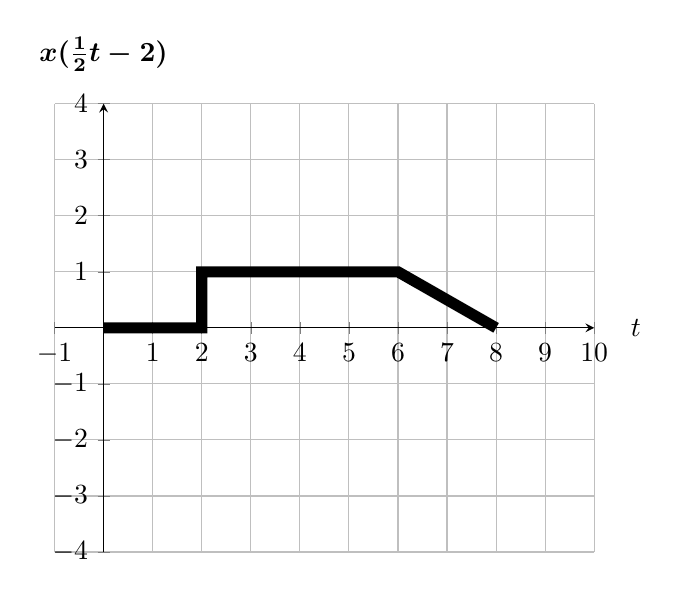
\begin{tikzpicture}[scale=1.0]
           \begin{axis}[
          axis lines=middle,
          xlabel={$t$},
          ylabel={$\boldsymbol{x(\frac{1}{2}t-2)}$},
          xtick={-1, ..., 10},
          ytick={-4,-3,-2, -1, ..., 4},
          ymin=-4, ymax=4,
          xmin=-1, xmax=10,
          every axis x label/.style={at={(ticklabel* cs:1.05)}, anchor=west,},
          every axis y label/.style={at={(ticklabel* cs:1.05)}, anchor=south,},
          grid,
        ]
           \path[draw,line width=4pt] (0,0) -- (2,0) -- (2,1) -- (6,1) -- (8,0);
           \end{axis}
        \end{tikzpicture}
        \caption{$t$ vs. $x(\frac{1}{2}t-2) $.}
        \label{fig:q2}
    \end{figure}



\section*{Answer 3}
\subsection*{a)}
\[ \sum_{k=-3}^3 {x[k]  \delta [n-k]} \]
\[ = \delta [n+3] - \delta [n+2] - \delta [n+1] -  \delta [n] + \delta [n-1] + 2\delta [n-2] + \delta [n-3]   \]


\end{document}



\begin{document}



\end{document}
